% !TeX root = thesis_main.tex
% ---------------------------------------------------
% ----- Introduction of the template
% ----- for Bachelor-, Master thesis and class papers
% ---------------------------------------------------
%  Created by C. Müller-Birn on 2012-08-17, CC-BY-SA 3.0.
%  Last upadte: C. Müller-Birn 2015-11-27 
%  Freie Universität Berlin, Institute of Computer Science, Human Centered Computing. 
%
\chapter{Introduction}
\label{chap:introduction}

\section{Topic and context}

In the ever-growing world of software development, many companies are now in the situation to maintain a large software ecosystem with complex dependencies.
Still, there is need for continuous improvement and development to stay competitive.
% but still want to improve their systems by developing new components and tools.
This poses the challenge of improving the software from aspects like user experience, scalability and maintainability while being restricted by the ecosystem.
\\
From my point of view, \Gls{greenfield} seems to be implicitly assumed in many books and articles about HCI.
This assumption is not applicable to the situation many software companies are in today.
\\
In a brownfield project, HCI methods need to be adapted to account for technical constraints while still addressing user needs. This approach was taken during the design and development of the UI Editor in this thesis.
In addition, user research in general is often neglected due to tight deadlines and limited resources which usually leads to premature releases and unstable software.

\section{Goals of this thesis}
The goal is to demonstrate how HCI principles and methods can be applied in a brownfield project, using a real-world case study at the company Sprylab as an example.
Sprylab is a company which is engaged in the digital publishing industry, providing \Gls{saas} to publishing houses for editing and distributing content.
% Intro UI Editor
The case study consists of the redevelopment of a UI Editor to improve user experience and usability for web developers, admins and editors.

\newpage
\section{Process for research, prototyping and implementation}

The software design process used to develop the Editor is described in \cite[p. 104]{LearnHCI:2020ys}.
There, the process is divided into the three phases "\Gls{design-thinking}", "\Gls{lean-ux}" and "\Gls{agile}".

For this concrete case study, the process looks like this:
\begin{figure}[h]
  \centering
  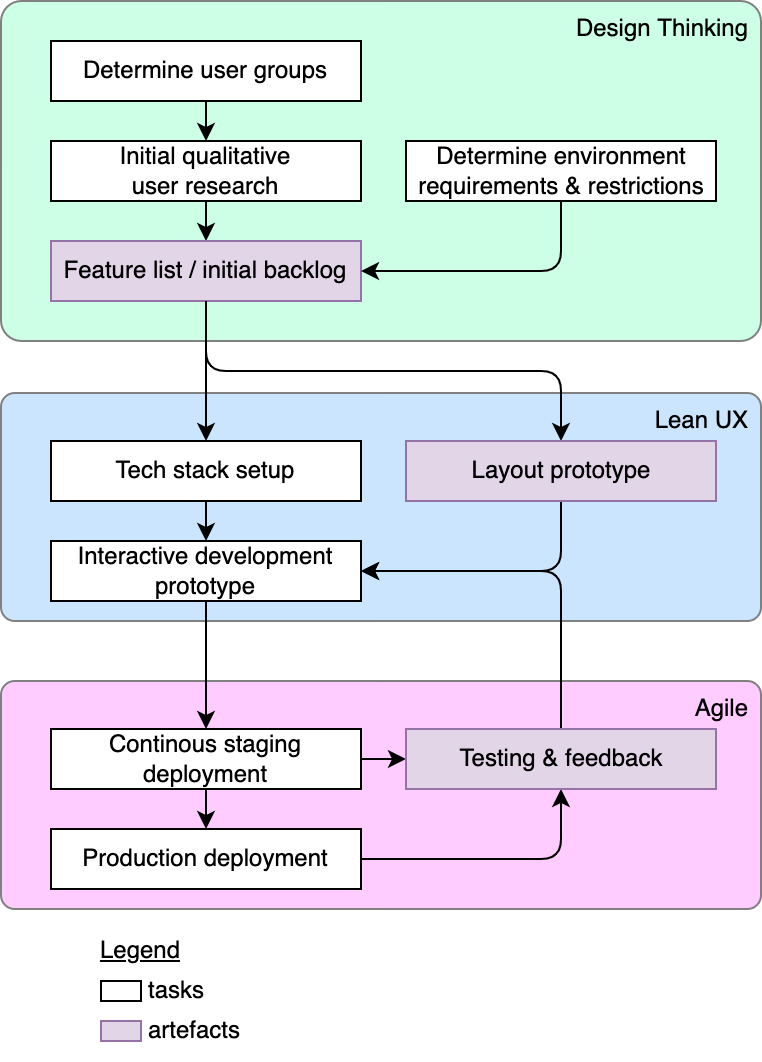
\includegraphics[width=0.8\linewidth]{pics/process.drawio.png}
  \caption{Software design process for the UI Editor.}
	\label{fig:process}
\end{figure}

